\documentclass[answers,addpoints]{exam}
\usepackage[margin=10mm]{geometry}
\usepackage{amsthm}
\usepackage{float} %  figure inside minipage 
\usepackage{ifthen,empheq}
\usepackage[]{graphicx}
\usepackage[]{minted}
\usepackage{amssymb}
\usepackage[multidot]{grffile}
\usepackage{pgfplots}
\usepackage{pgfplotstable}
\setlength{\headheight}{20pt}

\usepackage{tikz}
\usepgfplotslibrary{external}
\tikzexternalize[prefix=_tikz/,shell escape=-shell-escape]
\tikzset{external/system call={pdflatex \tikzexternalcheckshellescape -halt-on-error -interaction=batchmode -jobname "\image" "\texsource"}}
\immediate\write18{mkdir -p _tikz}

\title{Solution to HW2}
\author{Dilawar Singh}
\usepackage{hyperref}

\begin{document}
\Large
\maketitle

\begin{questions}

    \question[20]

    Refer to homework statement.

    \begin{solution}

        Except for the last subplot, these plots shows how each function
        will transform given functions in homework. These two functions are in
        first subplot. They are called \texttt{fun1} and \texttt{fun2}.

        \begin{figure}[H]
        \begin{center}
            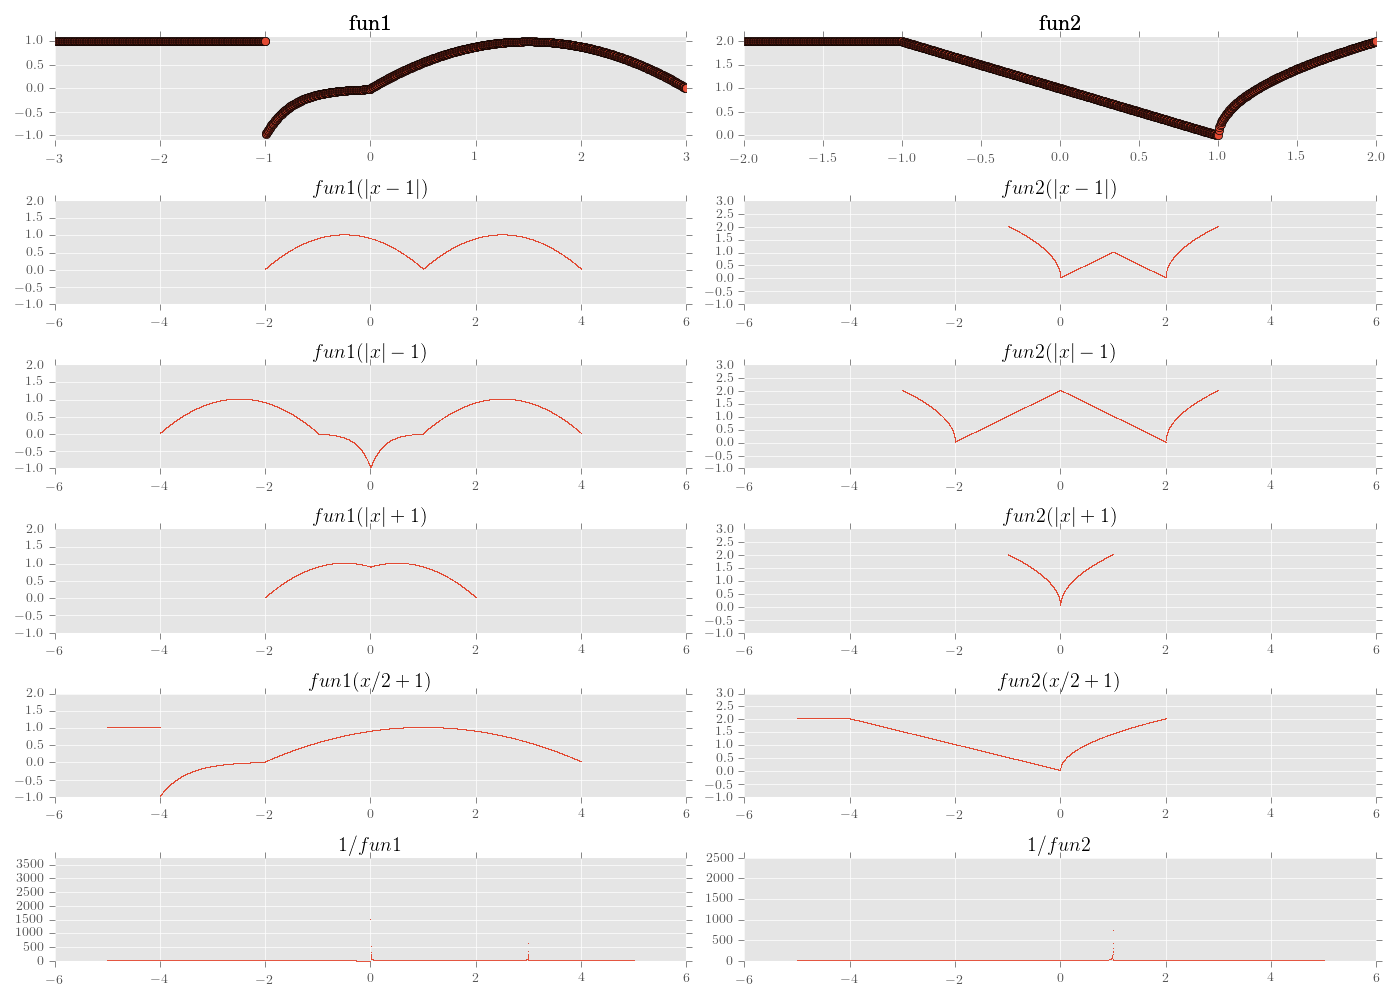
\includegraphics[width=1\textwidth]{./solution1.png}
        \end{center}
        \caption{Solution to problem 1}
        \label{fig:}
        \end{figure}

    \end{solution}

    \question[12]
    Refer to homework statement.

    \begin{solution}

        See figure \ref{fig:sol2}.

        \begin{figure}[H]
            \begin{center}
                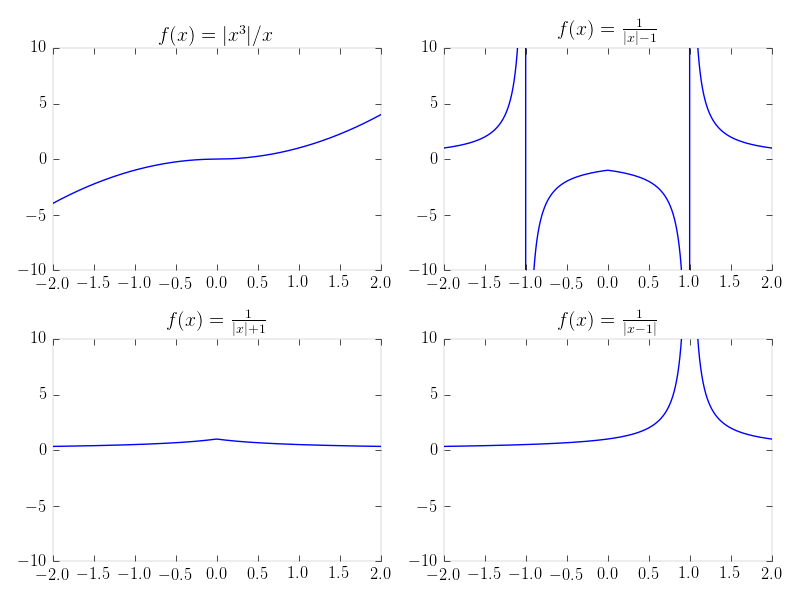
\includegraphics[width=1\textwidth]{solution2.png}
            \end{center}
            \caption{Solution 2}
            \label{fig:sol2}
        \end{figure}

    \end{solution}

    \question[5]

    Show that if $f(x) = \sqrt[3]{x}$, then for any $a \in \mathbb{R} \setminus
    \{0\}\; f'(a) = 1/3a^{-2/3}$.

    \begin{solution}

        We start with $f(a+h) = f(a) + h f'(a) + R(h)$ and $R(h)/h
        \rightarrow 0$ when $h \rightarrow 0$. We can write the following:

        \begin{align}
            f'(a)  = \lim_{h \rightarrow 0} \frac{ f(a+h) - f(a) }{h}  
        \end{align}

        This leads to,

        \begin{align}
            f(\sqrt[3]{x}) &= \lim_{h \rightarrow 0} \frac{ \sqrt[3]{x+h} - \sqrt[3]{x} }{h}  \\
                           &= \lim_{h \rightarrow 0} \frac{ (x+h)^{1/3} - x^{1/3} }{h} \\
                           &= \lim_{h \rightarrow 0} \frac{ x^{1/3} \left( 
        \left( 1 + \frac{h}{x}  \right)^{1/3} -1 \right)  }{h}
                           &= \lim_{h \rightarrow 0} \frac{ x^{1/3} \left( 
        1 + \frac{h}{3x} + \ldots  -1 \right)  }{h} \\
                            &= x^{1/3} \left( \frac{h}{3xh} \right) \\
                            &= x^{-2/3} \left( \frac{1}{3} \right) 
        \end{align}


    \end{solution}

\end{questions}

\end{document}          
